\documentclass[10pt,a4paper]{report}
\usepackage[utf8]{inputenc}
\usepackage{amsmath}
\usepackage{amsfonts}
\usepackage{amssymb}
\usepackage{graphicx}
\usepackage{lmodern}
\usepackage{float}
\usepackage[left=2cm,right=2cm,top=2cm,bottom=2cm]{geometry}
\begin{document}
\author{Yapi Donatien Achou}
\title{ex27}
\maketitle
\section{Setting up the problem}
\[
 u^{\prime\prime}(x) =
  \begin{cases}
   1 & \text{if } x < 1/2 \\
   0       & \text{if } x \ge 1/2
  \end{cases}
\]

with boundary condition
\begin{equation}
u(0) = u(1) = 0 \nonumber
\end{equation}

and basis functions
\begin{equation}
V = span\{\sin((i+1)\pi x)\} \nonumber
\end{equation}

\section{Galerkin method without integration by part}
In the Galerkin method we let the trial and the test function $u,v$ be in the space $V$:
\begin{equation}
u,v\in V\nonumber
\end{equation}
so that 
\begin{equation}
u = \sum{c_{i}\phi_{i}(x)} \nonumber
\end{equation}

\begin{equation}
v = \phi_{j}(x)\nonumber
\end{equation}

Our variational problem becomes
find $u\in V$ such that
\begin{equation}
\int_{0}^{\frac{1}{2}}\phi_{i}^{\prime\prime}\phi_{j}\mathrm{d}x\sum{c_{j}}= \int_{0}^{\frac{1}{2}}\phi_{j}\mathrm{d}x\nonumber
\end{equation}

without integration by part we have 
\begin{equation}
A_{ij} = \int_{0}^{\frac{1}{2}}\phi_{i}^{\prime\prime}\phi_{j}\mathrm{d}x \nonumber
\end{equation}

\begin{equation}
b_{j} = \int_{0}^{\frac{1}{2}}\phi_{j}\mathrm{d}x\nonumber
\end{equation}

The matrix $A$ is no longer symetric and is in fact singular

\section{Solution with P1 elements}
\begin{equation}
A_{ij} = \int_{0}^{\frac{1}{2}}\phi_{i}^{\prime}\phi_{j}^{\prime}\mathrm{d}x \nonumber
\end{equation}

\begin{equation}
b_{j} = \int_{0}^{\frac{1}{2}}\phi_{j}\mathrm{d}x\nonumber
\end{equation}

The analytical solution satisfying the boundary condition is  


\[
 u(x) =
  \begin{cases}
   \frac{1}{2}x^{2}-\frac{1}{2}x & \text{if } x < 1/2 \\
   0       & \text{if } x \ge 1/2
  \end{cases}
\]

therefore the solution is only non trivial in $(0,\frac{1}{2})$. The derivatives of the basis function are: 

\[
 \varphi_{i}^{\prime}(x) =
  \begin{cases}
   0 & \text{if } x < x_{i-1} \\
   \frac{1}{h}       & \text{if } x_{i-1} \leq  x < x_{i}\\
   -\frac{1}{h}      & \text{if } x_{i} \leq  x < x_{i+1}\\
   0     & \text{if }   x \ge x_{i+1}
  \end{cases}
\]

the solutions for $n=2,4,8$ are given bellow:

\begin{figure}[H]
  \caption{solution for $n= 2$}
  \centering
    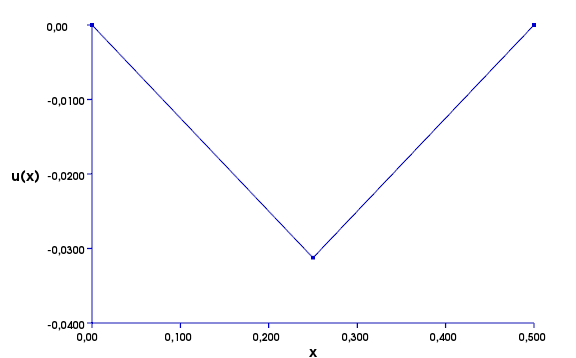
\includegraphics[width=0.5\textwidth]{n2.png}
\end{figure}

\begin{figure}[H]
  \caption{solution for $n= 4$}
  \centering
    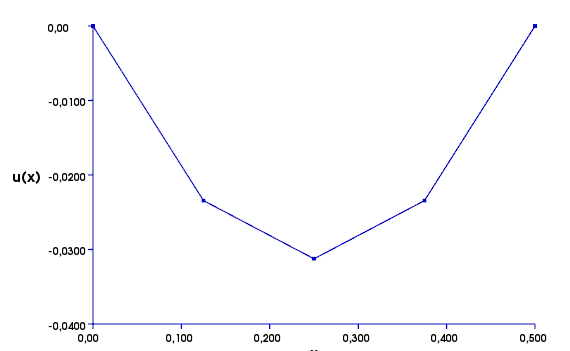
\includegraphics[width=0.5\textwidth]{n4.png}
\end{figure}

\begin{figure}[H]
  \caption{solution for $n= 8$}
  \centering
    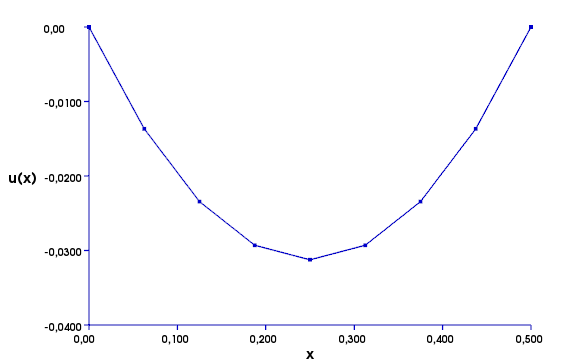
\includegraphics[width=0.5\textwidth]{n8.png}
\end{figure}
\end{document}